% -*- TeX-master: "../dipole_ilya_paper.tex" -*-
%%%%%%%%%%%%%%%%%%%%%%%%%%%%%%%%%%%%%%%%%%%%%%%%%%%%%%%%%%%%%%%%%%%%%%%%%%%%%%%%%%%% 
% kbordermatrix MUSE  BE PLACED IN /usr/local/texlive/2016/texmf-dist/tex/latex/base  and then
% run sudo -s texhash to load it up
%%%%%%%%%%%%%%%%%%%%%%%%%%%%%%%%%%%%%%%%%%%%%%%%%%%%%%%%%%%%%%%%%%%%%%%%%%%%%%%%%%%%

\documentclass[%
 reprint,
%superscriptaddress,
%groupedaddress,
%unsortedaddress,
%runinaddress,
%frontmatterverbose, 
%preprint,
%preprintnumbers,
%nofootinbib,
%nobibnotes,
%bibnotes,
 amsmath,amssymb,
 aps,
 prl
%pra,
%prb,
%rmp,
%prstab,
%prstper,
%floatfix,
 ]{revtex4-1}

%%% Geometry
\usepackage{geometry}
\geometry{top=25mm}
\geometry{bottom=35mm}
\geometry{left=30mm}
\geometry{right=20mm}
\usepackage{setspace}
\usepackage[toc,page]{appendix}

%%% Common Packages
\usepackage[usenames,dvipsnames,svgnames,table,rgb]{xcolor} % for colouring \color{red!20}
\usepackage{graphicx}       	% to include image
% \usepackage{caption}        	% image captions
\usepackage{framed}         	% \begin{framed} for framed boxes
\usepackage{multirow}               % merge rows in tables
\usepackage{bm}

%%% Maths settings
\usepackage{amsmath,amsfonts,amssymb,amsthm,mathtools} % all mathematical fonts
\usepackage{mathdots}               % to use \udots
\usepackage{esint}                      % fancy integrals
\mathtoolsset{showonlyrefs=true}        % only label formulas with references
\usepackage{comma}          	% smart comma spacing e.g $0,3$ becomes a list $0, 3$
\relpenalty=9999                        % prevent splitting of equations

%%% Physics Packages
\usepackage{qcircuit}               % for quantum circuits
\usepackage{braket}                 % \Bra and \Ket

%%% Images with Inkscape (they are used by it)
\usepackage{xifthen}
% \usepackage{pdfpages}
\usepackage{transparent}
\usepackage{import}

%%% URLS and Links
\usepackage{url}                    % add url in bibliography
\usepackage{hyperref}               % linking within document \hyperref[label]{text}

%%% PDF Metadata and colour
\hypersetup{
  unicode=true,
  pdftitle={},
  pdfauthor={Ilya   Antonov},
  pdfsubject={},
  pdfcreator={Ilya Antonov},
  pdfkeywords={} {} {},
  colorlinks=true,                      % links in color (true) or boxes (false)
  linkcolor=black,                      % internal links
  citecolor=blue!30,                    % bib links
  filecolor=magenta!20,                 % file links
  urlcolor=cyan                         % url links
}

%%% COLOURS
\newcommand{\red}[1]{{\color{red}{#1}}}
\newcommand{\blue}[1]{\textcolor{blue}{#1}}
\newcommand{\green}[1]{\textcolor{green}{#1}}
\newcommand{\purple}[1]{\textcolor{purple}{#1}}
\newcommand{\grey}[1]{{\color{gray!60} #1}}
\newcommand{\ec}{ }                             % end colour command for emacs regexp
\definecolor{amber}{rgb}{1.0, 0.75, 0.0}
\newcommand{\gold}[1]{{\color{amber}{#1}}}

%%% Physics
% Bra and Ket
\newcommand{\iket}[1]{\ensuremath{\Ket{#1}}}
\newcommand{\ibra}[1]{\ensuremath{\Bra{#1}}}
\newcommand{\iketbra}[2]{\ket{#1}\bra{#2}}
\newcommand{\iup}{\ensuremath{\Ket{\uparrow}}}
\newcommand{\idown}{\ensuremath{\Ket{\downarrow}}}
\newcommand{\iupBra}{\ensuremath{\Bra{\uparrow}}}
\newcommand{\idownBra}{\ensuremath{\Bra{\downarrow}}}
\newcommand{\iupKetBra}{\ensuremath{\Ket{\uparrow}\Bra{\uparrow}}}
\newcommand{\idownKetBra}{\ensuremath{\Ket{\downarrow}\Bra{\downarrow}}}
% matrices
\newcommand{\iz}{\ensuremath{\begin{pmatrix}1&0\\0&-1\end{pmatrix}}}
\newcommand{\ix}{\ensuremath{\begin{pmatrix}0&1\\1&0\end{pmatrix}}}
\newcommand{\iy}{\ensuremath{\begin{pmatrix}0&-i\\i&0\end{pmatrix}}}
\newcommand{\idensity}{\ensuremath{\begin{pmatrix}{\rho_{00}} & {\rho_{01}}\\{\rho_{10}}&{\rho_{11}}\end{pmatrix}}}

% symbols
\newcommand{\isigma}{\ensuremath{\vec{\iaverage{\sigma}}}}
\newcommand{\isigmax}{\ensuremath{{\iaverage{\sigma_x}}}}
\newcommand{\isigmay}{\ensuremath{{\iaverage{\sigma_y}}}}
\newcommand{\isigmaz}{\ensuremath{{\iaverage{\sigma_z}}}}
\newcommand{\iadagger}{\ensuremath{a^{\dagger}}}
\newcommand{\isigmaplus}{\ensuremath{\iaverage{\sigma^{+}}}}
\newcommand{\isigmaminus}{\ensuremath{\iaverage{\sigma^{-}}}}
\newcommand{\isigmaplusminus}{\ensuremath{\iaverage{\sigma^{\pm}}}}


%%% Math simplicity
\newcommand{\iunit}[2]{\ensuremath{#1\,\text{#2}}}
\newcommand{\iunitMixed}[3]{\ensuremath{#1\,#2\text{#3}}}
\newcommand{\iabsSquared}[1]{\ensuremath{\left|#1\right|^2}}
\newcommand{\iabs}[1]{\ensuremath{\left|#1\right|}}
\newcommand{\icommutation}[2]{\ensuremath{\left[#1,                                #2\right]}}
\newcommand{\iaverage}[1]{\ensuremath{\left\langle #1 \right\rangle}}
\newcommand{\iderivative}[2]{%
  \ensuremath{%
    \frac{\partial#1}{\partial#2}}}
\newcommand{\ira}{\ensuremath{\,\rightarrow\,}}
\newcommand{\iRa}{\ensuremath{\qquad\Rightarrow\qquad}}
\newcommand{\ilra}{\ensuremath{\,\leftrightarrow\,}}
\newcommand{\iratext}[1]{\ensuremath{\,\xrightarrow{\text{#1}}\,}}

\newcommand{\ialigned}[1]{\ensuremath{\left\lbrace\begin{aligned}#1\end{aligned}\right.}}
\newcommand{\ipic}[2]{\begin{center} \includegraphics[height=#1]{#2}
  \end{center}}
\newcommand{\ipicCaption}[3]{\begin{figure}[!ht]
    \begin{center}
      \includegraphics[height=#1]{#2}
      \caption{\small#3}
    \end{center}
  \end{figure}}
\newcommand{\iframe}[1]{\begin{framed}#1\end{framed}}
\newcommand{\ra}{\ensuremath{\rightarrow}}
\newcommand{\lra}{\ensuremath{\,\leftrightarrow\,}}
\newcommand{\ketbra}[2]{%
  \ket{#1}\bra{#2}%
}
\newcommand{\ia}{\ensuremath{a}}
\newcommand{\imatrix}[4]{\ensuremath{\begin{pmatrix}#1&#2\\#3&#4\end{pmatrix}}}
\newcommand{\xpi}{\ensuremath{\pi}}
\newcommand{\irho}[1]{\ensuremath{\rho_{#1}}}
\newcommand{\igamma}[1]{\ensuremath{\Gamma_{#1}}}
\newcommand{\iconjugate}[1]{\ensuremath{#1^{*}}}
\newcommand{\difffrac}[2]{%
  \ensuremath{%
    \frac{\partial#1}{\partial#2}}}
\newcommand{\iright}{\ensuremath{\quad\Rightarrow\quad}}
\newcommand{\imx}[4]{\ensuremath{\begin{pmatrix}#1&#2\\#3&#4\end{pmatrix}}}
\newcommand{\ifigure}[2]{\centering\makebox[\columnwidth][c]{\includegraphics[height=#1]{#2}}}


\begin{document}

%%% Title
\title{Primary insights into the superconducting twin qubit}

%%% Author
\author{I.  V.  Antonov}  \affiliation{Royal Holloway, University of London,  Egham, TW20 0EX,
  UK} \affiliation{National Physical Laboratory, Hampton Road Teddington, TW11 0LW, UK}

\author{R. S.  Shaikhaidarov}  \affiliation{Royal Holloway, University of  London, Egham, TW20
  0EX, UK}

\author{V.  N.  Antonov}  \affiliation{Royal Holloway, University of London,  Egham, TW20 0EX,
  UK}  \affiliation{Skolkovo Institute  of  Science  and Technology,  Nobel  str.  3,  Moscow,
  143026, Russia}  \affiliation{Moscow Institute  of Physics  and Technology,  29 Institutskiy
  per., 141700 Dolgoprudny, Moscow Region, Russia}

\author{O.V.  Astafiev}  \affiliation{Royal Holloway, University  of London, Egham,  TW20 0EX,
  UK}  \affiliation{Skolkovo Institute  of  Science  and Technology,  Nobel  str.  3,  Moscow,
  143026,  Russia} \affiliation{National  Physical Laboratory,  Hampton Road  Teddington, TW11
  0LW, UK}

\date{\today}

% -*- TeX-master: "../dipole_ilya_paper.tex" -*-

\begin{abstract}
  \noindent  A platform  of quantum  computation  based on  superconducting qubits  is on the
  verge of realization,  owing to the scalability and breadth  of 
  nanofabrication  technology.    However  the  latter has to  be set against their
  limited capability  of handling  sequential state operations. The  most successful
  processor prototype  has a decoherence time  of \iunit{\sim 60}{$\mu$s} while  each gate  is about  \iunit{20}{$\mu$s}. Therefore,  within 3  gate operations  it’s quantum  state
  becomes  substantially deteriorated.   Thus  short decoherence  time stands  as  a limiting factor of implementing superconducting quantum processors.

  % \noindent Short decoherence times stand as one of the main obstacles hindering industrial
  % scale implementation of quantum processors based on superconducting qubits.  The
  % simplicity
  % and flexibility of fabricating superconducting qubits compared with other qubit
  % architectures, most notably trapped ions, has to be set against their limited ability of
  % handling sequential state operations - the most successful processor prototype has a
  % decoherence time of $ \sim\iunitMixed{60}{\mu}{s} $ while the gate operation time is about
  % $\si\iunitMixed{20}{\mu}{s}$ \cite{linke2017}.  Therefore, within 3 gate operations it's
  % quantum state becomes substantially deteriorated.
  
  % Right now, in the embryonic stages of quantum infrastructure development, probability
  % theory
  % of the multi-armed bandit dictates \cite{gittins1989}: to maximize expected gains in
  % combating this decoherence problem, resources should be allocated to exploring new
  % alternatives, as opposed to exploiting the possibly sub-optimal (requiring a supporting
  % qubit overhead that is double the size of the original system) error correction mechanism
  % already in place \cite{reed2011}.
  
  In this work we look  at a new ``twin-qubit'' geometry - a fusion  of two flux qubits joined
  by a  common Josephson Junction, which  can potentially outperform current  devices.  At the
  degeneracy flux-bias  point, $  \Phi_0/2 $, the  twin qubit has  energy spectrum  plateaus with
  curvature  several orders  of magnitude  lower than  that in  the usual  flux qubits.   This
  flatness makes the qubit more robust to flux noise.  Also, the new qubit allows the \iket{1}
  \ilra \iket{2}  dipole transition  at the aforementioned  degeneracy point,  where coherence
  time is longest. This transition is forbidden in other qubit designs.
  % , and under the most basic of fabrication cycles, the
  % qubit demonstrates a decoherence
  % time of 42\,ns.
  We experimentally study the new qubit, get the transmission spectrum, Rabi oscillations, and
  fully simulate  the operation of  the qubit.
\end{abstract}

%%% Local Variables:
%%% mode: latex
%%% TeX-master: "../dipole_ilya_paper"
%%% End:


\maketitle

% -*- TeX-master: "../dipole_ilya_paper.tex" -*-

\section{Introduction}
% A  quantum   electronic  platform   that  parallels  the   functionality  of   a  transistor
% \cite{Astafiev2010}\cite{hoi2011},    multiplexer   \cite{honigl2018}    and   serial    bus
% \cite{shen2005} will server  as an intergral part of commercialisation  of quantum computing
% power.  Superconducting quibts are one of the device sof choice

\noindent Superconducting  qubits are  one of  the promising  trends for  implementing quantum
computing technology. Typical qubits are  on-chip aluminum structures with Josephson junctions
(JJ), whose geometry can be designed to select an operating energy, state transition rates and
sensitivity required in a particular environment.  Over  the past decade they have carried out
the functionality of a transistor \cite{Astafiev2010, hoi2011}, where a control field was used
to pass or block  a second field at a different  frequency, multiplexer \cite{honigl2018}, two
input signals can  be mixed to controllably  generates a single output signal,  and serial bus
\cite{shen2005}.    Superconducting   qubits  can   be   produced   using  industry   standard
nanofabrication   techniques  and   integrated   at  scale   into   large  coherent   circuits
\cite{johnson2010}.   All speaks  to  a strong  case of  servicing  future quantum  electronic
platforms with this technology.

One of the inherent limitation superconducting  qubits face is a comparatively short coherence
time,   $\tau_{\text{dec}}$,    beyond   which    quantum   information   becomes    lost,   (see
Appendix~\ref{sec:decoh-results-loss}).  For example, the transmon qubits in the revolutionary
5-qubit                quantum                experience               from                IBM
(\href{http://www.research.ibm.com/ibm-q}{research.ibm.com/ibm-q})  have a  coherence time  of
only $  60\,\mu $s  \cite{linke2017}.  In  order to have  a sufficient  number of  quantum logic
operations for  multi-stage computations, say  $ 10^4 $, coherence  times need to  surpass the
$ 100\,\mu$s barrier.

Strong  decoherence  in  superconducting  qubits  is partially  a  consequence  of  the  large
capacitances  inherent to  their  geometry.   The superconducting  loops  in  flux qubits  are
typically  $  \iunitMixed{1}{\mu}{m}$ or  greater  in  size \cite{hoi2011,  johnson2010},  which
couples them to  charge variations in the external environment.   Such fluctuations modify the
qubit's energy levels, consequently leading to an erratic evolution of the quantum state which
`washes' out quantum information \cite{devoret2008}.
 
Particularly in  flux qubit architectures  the JJ energy  dominates over the  charging energy,
E$_J/$E$_C     >>     1$,     which     lowers     the     device's     charge     sensitivity
\cite{orlando1999,chiorescu2003,mooij1999}.  A whole family of flux qubit designs have lead to
improvement of the  coherence times: shunted flux qubit $\sim80\,\mu$s  \cite{yan2016} , 4-JJ qubit
\cite{qui2016}, fluxonium $\sim1\,$ms \cite{pop2014}.

Here we investigate experimentally a `twin'  qubit, consisting of two symmetrical flux qubits,
linked by a common $ \alpha-$Josephson Junction  (Fig.~\ref{fig:setup}).  A chain of 15 such qubits
was recently  placed into  a coplanar  waveguide to  demonstrate flux-tunable  transmission of
microwaves \cite{shulga2018}.  Of particular interest to us is the weak flux dependence of the
systems transition  energy when  it was  biased to the  degeneracy point  $\Phi_0/2 $,  making it
benefit from both low flux and charge sensitivities.
 
In this  work we  characterize the twin  qubit in  a way that  has not been  done before  - we
isolate one of  the qubits and realize  it's capacitive coupling to the  transmission line. We
provide the first experimentally measured transmission spectrum and find: strong anharmonicity
with respect  to the  \iket{1}\ilra\iket{2} and  \iket{2}\ilra\iket{3} transitions;  weak flux
dependence  of the  transition  energies close  to  the degeneracy  point;  compliance of  the
experimental   energy   spectrum   with   simulations  and   outstanding   features   of   the
\iket{1}~\ilra~\iket{2} dipole transition.


% tuneable capacitive coupling to the tranmission  line, resulting from a flux-tuneable dipole
% moment.


% -*- TeX-master: "../dipole_ilya_paper.tex" -*-
\section{Sample Details}

\begin{figure}[h]
  \centering\def\svgwidth{8.5cm}\import{images_inkscape/}{fig1.pdf_tex}
  \caption{\small  \textbf{Geometry  of a  twin  qubit:}  (a) Scanning  electron
    microscope image of the twin qubit. The Al-AlO$_x$-Al JJs are highlighted in
    red and  pink; (b) Each  of the qubits is  coupled to the  transmission line
    with a T-shaped  capacitor; (c) The twin qubit is  a symmetrical arrangement
    of two individual  flux qubits (as described  in \cite{orlando1999}) sharing
    the central  JJ.  Islands are labeled  with a Cooper pair  occupation n$_i$,
    phase $\varphi_i$ and voltage V$_i$, with the  ground setting a reference of 0 for
    all  three variables.   JJs  (marked with  crosses)  mediate capacitive  and
    Josephson  interactions between  the islands.
    % The central  junction has  a    capacitance  of  $\alpha$C  and  Josephson  energy  $  \alpha$E$_{J}$,  compared  with    C$_J$, E$_J$ of the outside ones
  }
  \label{fig:setup}
  
\end{figure}


%% Describe fabrication
\noindent The sample is fabricated on an undoped 100 silicon substrate, which is
pre-patterned with NiCr(10\,nm)-Au(90\,nm) ground planes. We  use an electron
beam lithographer and a shadow evaporation  technique to create the structure of
Fig.~\ref{fig:setup}. The qubit consits of five JJ junctions integrated into two
symmetrical  superconducting  loops.   The  JJ  have  a   layered  structure  of
Al\,(\iunit{20}{nm})\,-\,AlO$_{\text{x}}$\,(oxidized     for      10\,min     at
\iunit{0.3}{mbar})\,-\,Al(\iunit{30}{nm}).  The energy  and  capacitance of  the
central JJ  is a  factor of  $\alpha$ larger than  for the  outside ones,  which have
dimensions  \iunit{400\times200}{nm$^2$}.    The  coplanar  transmission   line  with
impedance $ Z_{0} \sim 50\,\Omega $ runs to the opening between the ground planes in the
center of the chip. The qubits are capacitively coupled to the transmission line
through T-shaped  capacitors.  Phase  biases $\varphi,  \eta \varphi$, are  applied to  the two
superconducting loops with an external magnetic field.


% We begin by cleaning the wafer for  $\sim$~10 minutes at 60\,C in acetone rinsing
% in de-ionized water.  Two layers of  electron resist are sequentially spun and
% post baked  (3\,minutes at 60\,C)  onto the wafer: {Copolymer  13\%}, 700\,nm;
% ZEP520a:Anisol 2:1,  60\,nm.  We use  an electron beam lithographer  to expose
% the   resist   using   a   30\,kV,   10\,pA  beam   delivering   a   dose   of
% $  70\,\mu  $C/cm$^2$.   The  exposed  pattern  is  developed  in  P-xylene  for
% 35\,seconds followed by a 5\,minute submersion in IPA:H$_2$0 93:7 and rinse in
% pure IPA.   Shadow evaporation  of aluminum (Al)  in a  Plassys simultaneously
% deposits the JJs and the transmission line.  Plasma cleaning with argon before
% the deposition of Al removes residual resist and ensures good galvanic contact
% to  the gold  pattern. Deposit  of 20\,nm  of Al  is carried  in situ  without
% breaking  of   vacuum  followed  by   static  oxidation  for  10   minutes  at
% 0.3\,mBar. The intermediate AlO$_x$ insulating  layer is formed at the surface
% of Al, which serves  as a tunnel barrier of the JJ.  A  second 30\,nm layer of
% Al completes the process.


% This is taken from the paper characterization and reduction of capacitive loss
% induced by sub-micron JJ fabrication in superconducting qubits

%% Describe setup
We mount our sample on a holder with a superconducting-coil magnet on the 13\,mK
stage of  a dilution refrigerator.  A  superconducting shield is used  to screen
the holder  from stray magnetic  fields.  The RF  lines connected to  the sample
have attenuators for thermalization: -50\,dBm on  the 50K stage, -30\,dBm on the
4\,K  stage.  We  attach a  circulator on  the output  line for  isolation.  The
transmitted signal is amplified  by +35\,dBm on the 4K stage  and by +35\,dBm at
room  temperature.  This  set  of attenuators  and  amplifiers facilitate  power
conversion  between the  laboratory equipment  and qubit  microwaves.  Prior  to
performing  characterization measurement,  we  took  the microwave  transmission
spectrum with the qubit detuned, and  normalize all measurements by the background
transmission profile.

Our primary goal  in the experiment was to study  the intrinsic energy structure
of  the  qubits  and  compare  it  with the  theory,  as  opposed  to  achieving
competitive performance. Fabrication did not to go to the depths of chemical and
physical treatment of  the substrate surface to remove  two-level system defects
in the  silicon oxide layer \cite{earnest2018}  and we did not  employ infra-red
filters to  eliminate stray  light during measurement  \cite{barends2011}. There
steps would nevertheless be crucial to further improve the parameters of the
qubit.

%%% Local Variables:
%%% mode: latex
%%% TeX-master: "../dipole_ilya_paper"
%%% End:



% -*- TeX-master: "../dipole_ilya_paper.tex" -*-
\section{Operations with qubits}
\label{sec:characterisation}

% \red{Need scattering data}

\noindent  We record  the energy  spectrum  of the  twin qubit  using a  network
analyzer,  while  sweeping  the  biasing  magnetic flux.   Because  of  a  small
asymmetry, $\eta$, the fluxes linked through  the left and right loops are slightly
different: $ \Phi = \frac{\varphi}{2\pi}\Phi_0$ and $ \eta\Phi $, where $\eta\approx1$.

The  \iket{1}~\ilra~\iket{2}  transition, $\omega_{21}$,  is  mapped  with a  network
analyzer which measures  the transmission of signal  $\omega_{\text{NA}}$ through the
system.  Away from  resonance the signal passes through the  circuit without any
interaction with the qubit.  After  correcting for the line losses, transmission
is close to  $ 100\% $.  Only near resonance  ($\omega_{\text{NA}}=\omega_{21}$), does the
qubit exchange photons  with the driving field as it  evolves between the ground
and excited states.  The  qubit emits a wave that is  exactly in anti-phase with
the driving  field \cite{abdumalikov2010}, and the  destructive superposition in
the output line results in  a transmission dip, see Fig.~\ref{fig:transmission}.
The trace of blue circles of  the transmission minima at different magnetic flux
maps   out   the   qubit's   $\omega_{21}$  transition   spectrum,   see   inset   of
Fig.~\ref{fig:transmission}.

\begin{figure}[h]
  \centering\def\svgwidth{9.5cm}\import{images_inkscape/}{fig2.pdf_tex}
  \caption{\small \textbf{Mapping  the qubit transition  spectrum:}  For the  lower transition
    $\omega_{21}$ (blue) a  network analyzer measures  the power  transmission coefficient,
    \iabsSquared{t}, at flux  bias $ \Phi $  and microwave frequency $  \omega_{21}/2\pi$.  A Lorentzian
    fit \cite{Astafiev2010}  to the transmission  profile establishes the  resonant frequency,
    which  is  marked  with  blue  points on  the  flux-frequency  spectrum.   For  transition
    $\omega_{32}$  (red)  a two-tone  measurement is  run by  monitoring changes  to a  weak
    $\omega_{21}$ probe while sweeping a second frequency  in search of the higher transition.
    % Any changes to the probe's transmission are indicative of hitting the higher transition, which
    % is marked with a red point on the spectrum.
    % Readings are taken about the degeneracy point
    % $  \Phi \sim  \Phi_{0}/2 $,  where the  low  curvature of  transition energies,  allows for  stable
    % measurements with respect to fluctuations in the field.
  }
  \label{fig:transmission}
\end{figure}

The  \iket{2}\ilra\iket{3}  transition,  $\omega_{32}$,   is  mapped  using  two-tone
spectroscopy.   The network  analyzer probes  signals at  $ \omega_{21}  $, while  an
additional generator  sweeps a second  frequency, $ \omega_{\text{GEN}}  $.  Whenever
the      generator     strikes      the     \iket{2}\ira\iket{3}      transition
($\omega_{\text{GEN}}  = \omega_{32}  $), the  qubit  undergoes a  ladder of  excitations,
\iket{1}  \iratext{$\omega_{21}$}\iket{2}  \iratext{$\omega_{32}$} \iket{3},  depopulating
states \iket{1} and \iket{2}.  Because of this depopulation, the probe signal is
no longer  absorbed to drive  the \iket{1}\ilra \iket{2} transmission,  and it's
transmission  moves out  of  the resonance  dip in  Fig.~\ref{fig:transmission}.
This identifies  $\omega_{32}$ which  is mapped  with red  circles in  the transition
energy-magnetic field spectrum.

% prove that state 1 becomes depopulated  by solving the master equation for two
% drives

We match the  experimental data points to simulations: Islands,  isolated by the
JJ  in  Fig.~\ref{fig:setup},  are  labeled with  Cooper  pair  (CP)  occupation
$       \vec{n}      =       \iket{n_1,      n_2,       n_3}      $,       phase
$     \vec{\varphi}     =     \iket{\varphi_1,     \varphi_2,     \varphi_3}     $     and     potential
$ \vec{V} = \iket{V_{1}, V_{2}, V_{3}}  $ states.  The charges and potentials on
the islands are linked by the capacitance matrix
\begin{equation}
  \label{eq:link}
  2e\vec{n} = \hat{C}\vec{V}.
\end{equation}

\noindent The capacitance matrix in the twin qubit topology is
\begin{equation}
  \label{eq:capac}
  \hat{C} = \iabs{C} \begin{pmatrix}
    2  &  -1  &  0\\
    -1  &  2  +  \alpha  &  -1\\
    0  &  -1  & 2
  \end{pmatrix},
\end{equation}

\noindent where \iabs{C}  is the capacitance of the outer  JJs.  The interaction
of the  CPs, carrying a  charge $ \vec{Q}=2e\vec{n}  $, and potentials  on their
respective islands gives rise to the `kinetic' term of the Hamiltonian:
\begin{equation}\label{eq:kinetic}
  \begin{aligned}
    T = \frac{1}{2}\sum_{i=1}^{3}Q_iV_i & =
    \frac{(2e)^2}{2}\vec{n}\hat{C}^{-1}\vec{n}^{T}\\
    & = E_C \iabs{C} \iaverage{\hat{C}^{-1}}_{\iket{n_{1}, n_2, n_3}},
  \end{aligned}
\end{equation}

\noindent where we define $ E_{C}={(2e)^{2}}/{2 \iabs{C} } $.

Each  JJ  with  a  phase  difference  of  $\Delta\varphi_{i}$,  contributes  an  energy  of
$ E_{Ji}\left(1 - \cos(\Delta\varphi_i)\right) $.   The flux quantization condition for the
left                     and                    right                     loops,
$ \sum_{i}^{\text{loop}}  \varphi_i = 2\pi  n, n \in \mathbb{Z}$,  enters as a  dependence on
$ \varphi_\text{ext} $ and $ \eta\varphi_\text{ext} $ on two of the junctions:
\begin{equation}\label{eq:potential}
  \begin{aligned}
    U & = E_J\big[4 + \alpha - \alpha\cos(\varphi_{2}) -\cos(\varphi_{1}) -\cos(\varphi_{3}) - \\
    &  \qquad  \cos(\varphi_{2}   -  \varphi_{1}  -  \varphi_{\text{ext}})  -  \cos(\varphi_{2}   -  \varphi_{3}  +
    \eta\varphi_{\text{ext}})\big].
  \end{aligned}
\end{equation}

The  Hamiltonian, $\mathcal{H}= T + U$, is  solved  in  the charge  basis (see  Appendix
\ref{sec:repr-hamilt-charge})  with
\iunit{E_J = 91.0}{GHz}, \iunit{E_C = 13.50}{GHz}, \iunit{\alpha = 1.023}{}, \iunit{\eta
  =    1.011}{}. The resulting eigenenergies   are    compared    with    the    experimental    ones    in
Fig.~\ref{fig:experiment} .  Data for $ \omega_{32} $ is taken in a narrow flux range
because away from $ \Phi = n \Phi_0, n\in\mathbb{Z} $, it gets harder to tune the VNA to
$ \omega_{21} $  in two-tone spectroscopy.  The  asymmetry value, $ \eta $,  is close to
the  visual   loop  area  difference  of   3\%  seen  from  the   SEM  image  in
Fig.~\ref{fig:setup}.  The  resonance is  periodic in flux,  with a  tendency of
higher $\omega_{21}$ at higher magnetic flux numbers.

\begin{figure}[h]
  % 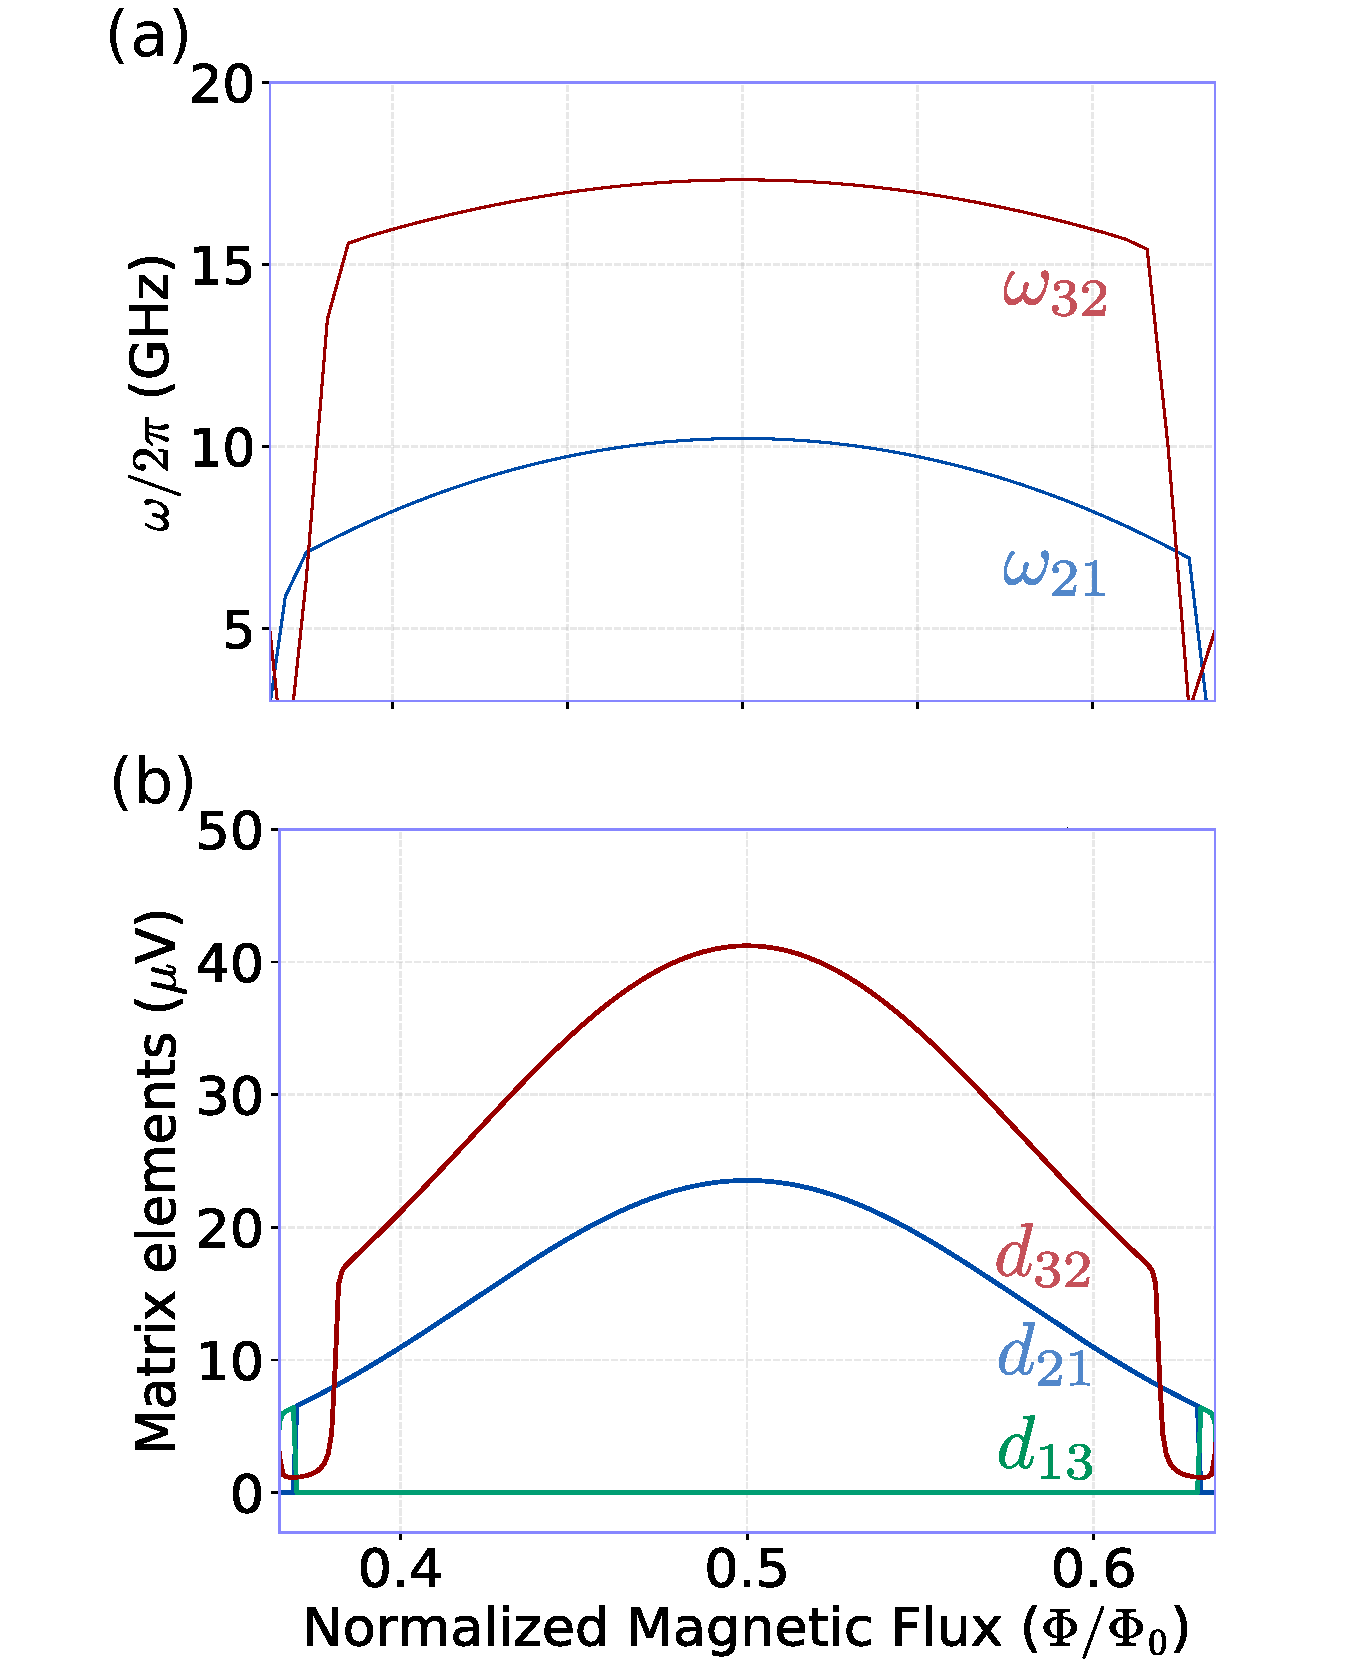
\includegraphics[width=8cm]{fig3}
  \centering\def\svgwidth{8cm}\import{images_inkscape/}{fig3.pdf_tex}
  \caption{\small \textbf{Experimental spectra, circles, and  simulation, solid lines, of the
      twin  qubit:}   Shown  are   the  transition   frequencies  $   \omega_{21}  $   (blue)  and
    $ \omega_{32}$ (red).  Asymmetry  in the flux penetrating the left and  right loops results in
    the  gradual   change  of   transition  frequencies   with  every   $  \Phi_{0}   $  period:
    $\omega_{21}$ creeps  up, while $\omega_{32}$ creeps  down, breaking the usual  periodicity of flux
    qubits.  \label{fig:experiment}}
\end{figure}
 
An  important qubit  parameter is  the curvature  at the  turning points  in the
energy  spectrum, at  the operation  point  of the  qubit.  A  low curvature  is
desirable, to  make the  qubit less  sensitive to  external flux  changes, which
would  improve  decoherence  time.   At   the  twin  qubits'  degeneracy  points
$      \Phi     =      n\Phi_0,     n\in\mathbb{Z}      $,     the      curvature     is
$   (-550\pm10)\,\text{GHz}/\Phi_0^2  $.    It   is   substantially  smaller   than
$  13\times  10^4$ $  \text{GHz}/\Phi_0^2$  on  the  4-JJ flux  qubit  \cite{stern2014},
$   8.4  \times   10^4\,   \text{GHz}/\Phi_0^2$  \cite{zhu2010}   and   $  37\times   10^{4}$
$ \text{GHz}/\Phi_0^2$  \cite{gustavsson2012} on the 3-JJ  flux qubits demonstrated
recently.  However,  the decoherence time  of $  = \iunit{42}{ns} $,  taken with
Rabi  oscillation   \cite{Bylander2011,Ithier2005,Martinis2003}  was  relatively
short, see  Fig.~\ref{fig:rabi}.  We attribute  this to poisoning of  the sample
with  the infrared  radiation, and  the  coupling two-level  oscillators in  the
substrate, owing to the simplified technology used in the qubit's fabrication.

\begin{figure}[h]
  % \includegraphics[width=8cm]{fig5}
  \centering\def\svgwidth{8cm}\import{images_inkscape/}{fig5.pdf_tex}
  \caption{\textbf{Rabi oscillations:}  taken at  the degeneracy point  by driving  the qubit
    with resonant microwaves pulses for fixed time periods, $ \Delta t $.  The decoherence time of
    $   \tau_{\text{dec}}  =   \iunit{42}{ns}  $   is   extracted  from   the  decay   envelope,
    $ e^{-\Delta t/\tau_{\text{dec}}} $, of the the oscillations. \label{fig:rabi}}
\end{figure}
  % Despite the twin qubit have a much the decoherence time
  % in our qubits was
  % relatively small This improved robustness to flux noise
  % is matched by a
  % decoherence time of , extracted from Rabi oscillations
  % in Fig.~\ref{fig:rabi}
  % \cite{rabi}.

%%% Local Variables:
%%% mode: latex
%%% TeX-master: "../dipole_ilya_paper"
%%% End:


% -*- TeX-master: "../dipole_ilya_paper.tex" -*-
\section{Dipole Transition}
\label{sec:dipole-transition}

\noindent  Finally we  characterize the  dipole moment  of transition  between the  lowest two
states,  \iket{1}   and  \iket{2}.   Microwaves   in  the  transmission  line,   with  voltage
$   V_{\text{mw}}=   \iabs{V_{\text{mw}}}\cos(\omega_{21   }t)   $  are   coupled   via   capacitor
C$_{\text{coupling}}$  to   the  qubit.   On   island  2   the  microwave  induces   a  charge
$ Q_{2}=C_{\text{coupling}}V_{\text{mw}} $.  Transitions \iket{1}~\ilra~\iket{2} stimulated by
this driving  generate a qubit voltage  of $ \delta  V_2 = \ibra{1}\hat{V}_2\iket{2} $  between the
ground and  island 2 and  hence draw an  electrostatic energy related  to the strength  of the
drive $\Omega$ by:
\begin{equation}
  \label{eq:dipoleEnergy}
  \begin{aligned}
    \delta V_{2}Q_{2} & = \ibra{1}\hat{V}_2\iket{2} C_{\text{coupling}}\iabs{V_{\text{mw}}}\cos(\omega_{21}  t) \\
    & = \hbar\Omega\cos(\omega_{21}t).
  \end{aligned}
\end{equation}

\noindent Thus, up to the constant of proportionality $ Q_{2} $, evaluation of
\begin{equation}
  \label{eq:dv2}
  \delta     V_2     =\ibra{1}\frac{E_{C}}{2\iabs{e}(1+\alpha)}\left[\hat{n}_1     +     2\hat{n}_2     +
    \hat{n}_3\right]\iket{2}
\end{equation}

\noindent gives the coupling strength $\Omega$ between  the microwave line and the qubit system. To
quantitatively compare coupling strength between  different flux qubit geometries, we re-write
the voltage element using flux:
\begin{equation}
  \label{eq:dipole_voltage_7}
  \begin{aligned}
    \ibra{1}\hat{V}_2 \iket{2} & =  \frac{d}{dt}\ibra{1}\hat{\Phi}_2\iket{2}\\
    & = \frac{d}{dt}\left[\left(e^{i\omega_{21}t/2}\ibra{1}\right) \hat{\Phi}_2\left(e^{+i\omega_{21}t/2}\iket{2}\right)\right]\\
    & = {i\omega_{21}\beta\Phi_0},
  \end{aligned}
\end{equation}

\noindent  In  the  last   equation  we  use  the  free  evolution   of  a  two-level  system,
$                   U(t)=e^{-i                    \frac{\mathcal{H}}{\hbar}t}                   $,
$  \mathcal{H}  =   -\frac{\hbar\omega_{21}}{2}\sigma_z  $,  to  draw  out  the   time-dependent  phases  in
$\delta  V_2$.   The  dimensionless  parameter  $\beta =  {\ibra{1}\hat{\Phi_2}\iket{2}}/{\Phi_0}  $  is  the
normalized coupling constant that can be compared across geometries.

In  Fig.~\ref{fig:fig5},  we  compare $\beta$  between  the  twin  qubit  and a  4-JJ  flux  qubit
\cite{honigl2018} .   Irrespective of  the energies  used in the  simulations, the  twin qubit
always has a  local maximum of coupling strength  at degeneracy points $ \Phi =  n\Phi_0$, while the
4-JJ coupling  strength goes  to zero.  We  have discussed earlier  the benefits  of operating
qubits  near the  degeneracy points  - where  there  is a  low magnetic  field sensitivity  to
magnetic field variations.  The twin qubit  allows \iket{1}\ilra \iket{2} transitions at these
optimal working points, while in other flux qubits this transitions are forbidden.

\begin{figure}[h]
  \centering\def\svgwidth{8cm}\import{images_inkscape/}{fig6.pdf_tex}
  % \centering \includegraphics[height=5cm]{fig6}
  \caption{\small \textbf{Dipole  coefficient:} Compared are the absolute magnitudes of $\iabs{\iabs{\beta}}$
    between the twin qubit (green) and 4-JJ (orange) qubit designs. In simulations we use $ \iunit{E_J =  91}{GHz}, \iunit{E_C  = 13.5}{GHz}, \iunit{\alpha  = 1.023}{},  \iunit{\eta =1.011}{} $ for the twin qubit and
    $ E_{C} = \iunit{20}{GHz}, E_J=\iunit{30}{GHz}, \alpha=0.45 $ for the 4-JJ qubit. The 4-JJ qubit has $\iabs{\beta} = 0$ in the vicinity of degeneracy points $  \Phi =  (n+\frac{1}{2})\Phi_0$, where the transition \iket{1} \ilra \iket{2} is therefore  forbidden.
    \label{fig:fig5}}
\end{figure}

% \begin{equation}\label{eqn:goldenRule}
%                                 \frac{1}{T_{21}}                              =
%                                 %                                 \frac{1}{Z_0}\hbar\omega_{21}\frac{\iabsSquared{\bra{2}T\iket{1}}}{\hbar^2}.
% \end{equation}

% \noindent The kinetic term  $ T $ plays the role of the  dipole operator for this transition
% and  is evaluated  with  the eigenstates  \iket{1}, \iket{2}  of  the Hamiltonian.   Highest
% transition      rates     are      achieved      around      the     degeneracy      biases,
% $  \varphi_{\text{ext}} =  (2n+1)\pi,  n\in\mathbb{Z} $,  see Fig.~\ref{fig:dipole_transition}.   This
% region is thus favourable for quick state operations with external driving fields.
 
% \begin{figure}
%   \centering 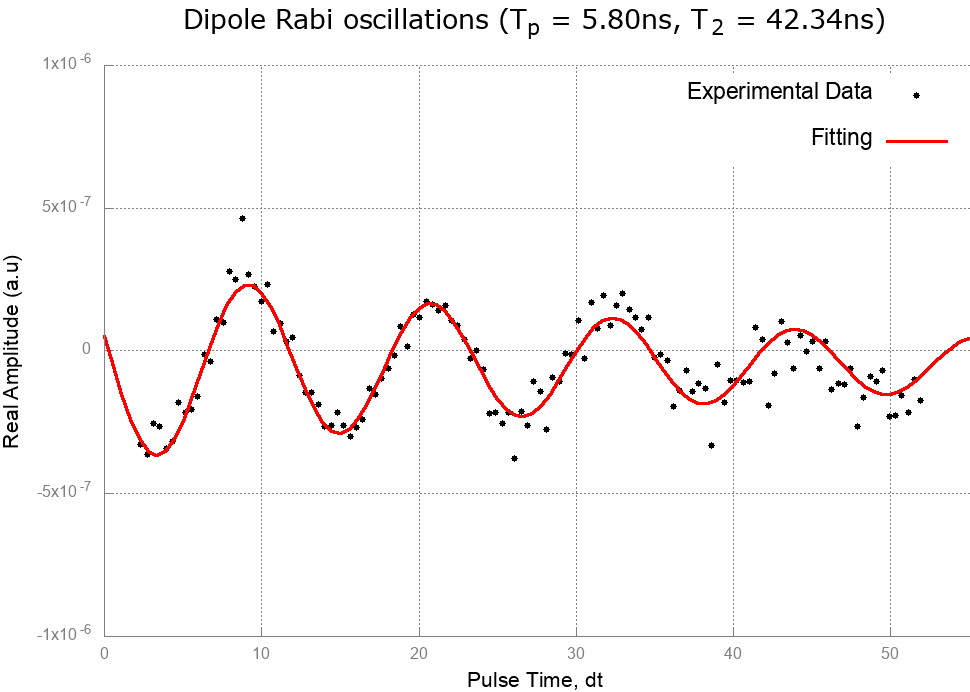
\includegraphics[height=6.5cm]{figure5.png}
 % 	\caption{The dipole transition rate $ \Gamma $ is proportional to the dipole transition element $ \bra{2}T\ket{1} $, where $ T $ is the charge operator responsible for the transition, and $ \iket{1} $ and \iket{2} are the eigenstates of the system. %There is strong transition between the levels at the turning point in magnetic flux, $ \Phi = (n+\frac{1}{2})\Phi_0, n\in\mathcal{Z} $.
 %  \label{fig:dipole_transition}}
 % \end{figure}

%%% Local Variables:
%%% mode: latex
%%% TeX-master: "../dipole_ilya_paper"
%%% End:


% -*- TeX-master: "../dipole_ilya_paper.tex" -*-
\section{Conclusion}
\noindent We  have fabricated and  characterized the first isolated  twin qubit.  It  has weak
flux  sensitivity  and   allows  \iket{1}\ilra  \iket{2}  transitions   at  degeneracy  points
$ \Phi =  n\Phi_0, n\in\mathbb{Z} $. The latter  effect is different from other flux  based qubits, where  this   transition  is  forbidden.   We   did  not  get  the   high  decoherence  times,
$\tau_{\text{dec}}$  is   only  \iunit{42}{ns},   but  it  can   be  substantially   improved  by
implementation of  advanced fabrication  techniques the  twin qubit may  be in  competition of
serving as the building block of quantum electronic circuits.


\noindent
%%% Local Variables:
%%% mode: latex
%%% TeX-master: "../dipole_ilya_paper"
%%% End:


\newpage
\begin{appendices}
  % -*- TeX-master: "../dipole_ilya_paper.tex" -*-

\section{Decoherence results in loss of quantum information}
\label{sec:decoh-results-loss}

\noindent Quantum  processing involves manipulating  the state of  a qubit, $\Psi$,  changing the
relative state population, $\ensuremath{|\alpha|} \le 1$, and phase, $\varphi$, between states \iket{0} and
\iket{1}:
\begin{equation}
  \label{eq:4}
  \Psi = \alpha\iket{0} + e^{i\varphi}(1-\alpha)\iket{1}.
\end{equation}

\noindent  When  written as  a  density  matrix, the  phase  information  is mapped  onto  the
off-diagonal elements:
\begin{equation}
  \label{eq:5}
  \rho = \iketbra{\Psi}{\Psi} = \begin{pmatrix}
    \iabsSquared{\alpha}  & \alpha(1-\alpha)e^{-i\varphi}\\
    \alpha(1-\alpha)e^{+i\varphi} & \iabsSquared{(1-\alpha)}.
  \end{pmatrix}
\end{equation}

\noindent Decoherence,  by definition, causes  the off-diagonal elements  decay to 1/e  of the
initial  value over  a time  $\tau_{\text{dec}}$. Decoherence  causes the  loss of  computational
information encoded in the phase $\varphi$.

\section{Representation of Hamiltonian in the charge basis}
\label{sec:repr-hamilt-charge}

\noindent The Hamiltonian

\begin{equation}
  \label{eq:hamitlian_revisited}
  \begin{aligned}
    \mathcal{H} & = T + U\\
    & = E_C \iabs{C} \iaverage{\hat{C}^{-1}}_{\iket{n_{1}, n_2, n_3}} \\
    & \quad+  E_J\big[4 + \alpha - \alpha\cos(\varphi_{2}) -\cos(\varphi_{1}) -\cos(\varphi_{3}) - \\
    &  \qquad  \cos(\varphi_{2}   -  \varphi_{1}  -  \varphi_{\text{ext}})  -  \cos(\varphi_{2}   -  \varphi_{3}  +
    \eta\varphi_{\text{ext}})\big]
  \end{aligned}
\end{equation}

\noindent in the charge basis  takes the  form  shown in  Fig.~\ref{fig:matrix_representation}, where a state \iket{-1, 0,  1} would correspond to a CP-occupation of -1, 0 and 1 on islands 1, 2 and 3.

Kinetic terms  ($ {T}  $) naturally  fall on  the diagonal  axis of  the matrix.
Potential terms ($  U $) are expanded to complex  exponentials, which become off
diagonal elements (see Appendix~\ref{sec:expans-potent-term}).

To decide on the number of states for the simulation, we took a sufficiently complete system state of 19 interacting CPs, and methodically ``switched off'' interactions between the high-CP-number states. I logged the deviation of the energy spectra of Fig.~\ref{fig:matrix_representation}, where it shows that 9-CP-states describes the system almost as well as with the complete system state.

\begin{figure}[h]
  \centering\def\svgwidth{8cm}\import{images_inkscape/}{fig4.pdf_tex}
  \caption{\small \textbf{Hamiltonian in the CP-basis representation for 3-CP-states-per-island (27 system states):} Purple square denote the kinetic terms that all fall on the main diagonal. Light blue squares denote simple off-diagonal terms distributed symmetrically about the main diagonal, arising from e.g. $\cos(\varphi_2)$. Dark blue squares are have an additional flux dependence $e^{i\varphi_{\text{ext}}}, e^{i\eta\varphi_{\text{ext}}}$, arising from e.g. $\cos(\varphi_2-\varphi_1-\varphi_{\text{ext}})$.
    \label{fig:matrix_representation} }
\end{figure}

\begin{figure}[h]
  \centering\def\svgwidth{8cm}\import{images_inkscape/}{fig7.pdf_tex}
  \caption{\small \textbf{Choosing the lowest number of interacting CP, that would  capture the nature of perturbation effects:} In the limiting case of too few CP-interactions (potential terms \,$U$\,), the full system states (19-CP) is substantially deviated from. At the sane tine, it made little sense to include more than 9 CP in the simulation.
    \label{fig:matrix_representation} }
\end{figure}

% For        example         $        \cos(\varphi_{2})         $        becomes
% $    \mathbb{I}_{1}\otimes\frac{1}{2}\left[\sum_{n_2}\iketbra{n_2+1}{n_2}    +
%   \iketbra{n_2-1}{n_2}   \right]\otimes\mathbb{I}_{3}    $,   where   identity
% operators $ \mathbb{I}_{1,3} $ carry the states of the non-involved islands.


\section{Expansion of potential term, $U$, in the CP-basis\label{sec:expans-potent-term}}

\noindent Switching to the CP-basis, leads  to a non-trivial representation of phase-dependent
terms in  $ U(\varphi_1,\varphi_2,\varphi_3,\varphi_{\text{ext}})  $.  The following  explanation will  illustrate the
expansion process.

\begin{enumerate}
\item Derive  the commutation relation  between the number, $  \hat{n} $, and  the exponential
  phase,     $    e^{\pm     i\hat{\varphi}}     $,    by     using     the    standard     relation
  $ \left[\hat{n},\hat{\varphi}\right] = 1 $:
 
  {\scriptsize\begin{equation}\label{eq:ab1}
      \begin{aligned}
        \icommutation{\hat{\red{n}}}{e^{\pm i \hat{\blue{\varphi}}}} & =  \icommutation{\hat{n}}{\sum_{\alpha = 0}^{\infty} \frac{(\pm i\hat{\blue{\varphi}})^\alpha}{\alpha!}} = \sum_{\alpha = 0}^{\infty} (\pm i)^\alpha\frac{\icommutation{\hat{\red{n}}}{\hat{\blue{\varphi}}^\alpha}}{\alpha!}\\
        &  = \sum_{\alpha  = 0}^{\infty}  (\pm i)^\alpha\frac{-\alpha  i\hat{\blue{\varphi}}^{\alpha -  1}}{\alpha!}  =  \pm \sum_{\alpha  =
          1}^{\infty}i^{\alpha  -  1}\frac{(\pm\hat{\blue{\varphi}})^{\alpha  -  1}}{(\alpha   -  1)!}   =  \pm  e^{\pm
          i\hat{\blue{\varphi}}}.
      \end{aligned}
    \end{equation}}

\item Operating with the number operator on state $ e^{\pm i\hat{\blue{\varphi}}}\ket{n} $ and using
  the commutation result \begin{equation}\label{eq:ab2}
    \begin{aligned}
      \hat{\red{n}}\bigg[e^{\pm   i\hat{\blue{\varphi}}}\ket{n}\bigg]    =   &    \bigg[\pm   e^{\pm
        i\hat{\blue{\varphi}}}   +  e^{\pm   i\hat{\blue{\varphi}}}\hat{n}\bigg]\ket{n}  \\   &  =   (n\pm
      1)\bigg[e^{\pm i\hat{\blue{\varphi}}}\ket{n}\bigg].
    \end{aligned}
  \end{equation}

\item Evidently, the exponential phase operator is a ladder operator for the \iket{n} state:
  \begin{equation}
    \label{eq:ab5}
    e^{\pm i\hat{\blue{\varphi}}}\ket{n} = \ket{n \pm 1} \Rightarrow e^{\pm i\blue{\varphi}} = \sum_{{n}} \iketbra{n\pm1}{n}.
  \end{equation}
 
\item Thus  operator $\cos(\hat{\varphi}_2-\hat{\varphi}_1-\hat{\varphi}_{\text{ext}})$ can be  expressed in the
  number basis $ \left\{n_{1},n_2,n_3\right\} $ as: {\scriptsize
    \begin{equation}
      \label{eq:ab4}
      \begin{aligned}
	\cos(\hat{\varphi}_2-& \hat{\varphi}_1-\hat{\varphi}_{\text{ext}}) =\\
        & = \frac{1}{2}\left(e^{i\hat{\varphi}_{2}}e^{-i\hat{\varphi}_1}e^{-i\hat{\varphi}_{\text{ext}}}+\text{c.c.}\right)\\
        & =  \frac{1}{2} \left(\left[\sum_{n_2}\iketbra{n_2+1}{n_2}\right]\right. \\
        & \qquad \left.\otimes \left[\sum_{n_1}\iketbra{n_1-1}{n_1}\right]
          \otimes\mathbb{I}^{(3)}\right)e^{-i\varphi_{\text{ext}}} + \text{c.c.}\\
        &             =              \frac{1}{2}e^{-i\varphi_{\text{ext}}}             \sum_{n_{1,2,3}}
        \iketbra{n_1-1,n_2+1,n_3}{n_1,n_2,n_3} + \text{c.c.}
      \end{aligned}
    \end{equation}}
  
\item Physically this corresponds  to a CP exchange between island 1 and  island 2. An example
  of a term could be
  \begin{equation}
    \label{eq:ab6}
    \frac{1}{2}e^{-i\varphi_{\text{ext}}}\iketbra{-1,1,0}{0,0,0} + \frac{1}{2}e^{+i\varphi_{\text{ext}}}\iketbra{0,0,0}{-1,1,0},
  \end{equation}
  \noindent  which would  be a  pair of  symmetrical off-diagonal  elements in  the matrix  of
  Fig.~\ref{fig:matrix_representation}.
\end{enumerate}


% \section{Rabi oscillation measurements}
% \label{sec:rabi-oscill-meas}

% \noindent Rabi  oscillations are observed when  a qubit system, with  a transition frequency
% $\omega_{21}$, is driven by microwaves in  resonance with this transition.  The expectation value
% of  $ \iaverage{\sigma_{-}}  $, $\sigma_{-}=\iketbra{0}{1}$,  which is  measured by  a vector  network
% analyzer \cite{Astafiev2010}, oscillates sinusoidally with the  length of the drive as shown
% below.

% \begin{enumerate}
% \item The Hamiltonian during microwave driving of the system is a combination of the qubit's
%   two-level system Hamiltonian
%   \begin{equation}
%     \label{eq:rabi1}
%     \mathcal{H}_{q} = -\frac{\hbar\omega_{21}}{2}\sigma_{z},
%   \end{equation}

%   \noindent                                                                            where
%   $\sigma_z = \ensuremath{\left(\begin{smallmatrix} 1  & 0\\0 & -1 \end{smallmatrix}\right)}
%   $, and the Hamiltonian of the resonant drive of strength $ \hbar\Omega $
%   \begin{equation}
%     \label{eq:rabi2}
%     \mathcal{H}_{d} = \hbar\Omega\cos(\omega_{21}t)\sigma_{x}
%   \end{equation}

%   \noindent   that    couples   the   two    levels   through   the    transition   operator
%   $\sigma_x = \ensuremath{\left(\begin{smallmatrix} 0 & 1 \\ 1 & 0 \end{smallmatrix}\right)}
%   $.

% \item              Applying              the             unitary              transformation
%   $     U(t)    =     \exp    \left(-i     \frac{\omega_{21}t}{2}\sigma_z\right)    $     to
%   $ \mathcal{H} = \mathcal{H}_{q}+\mathcal{H}_{d} $ evaluates to
%   \begin{equation}
%     \label{eq:rabi3}
%     \begin{aligned}
%       \mathcal{H}'& = U\mathcal{H}U^{\dag} - i\hbar U\dot{U}^{\dag}\\
%       & \approx \frac{\hbar\Omega}{2}\sigma_x
%     \end{aligned}
%   \end{equation}

%   \noindent    under     the    approximation     that    non-conserving     energy    terms
%   $ e^{\pm 2i\omega_{21}t} $ are neglected.
  
% \item  The evolution  of  a  ground state  in  this  rotated frame  for  a  drive of  length
%   $ \Delta t $ is
%   \begin{equation}
%     \label{eq:rabi4}
%     \begin{aligned}
%       U'(\Delta t)\iket{0} & = e^{-i\frac{\mathcal{H'}}{\hbar}\Delta t}\iket{0} \\
%       &     =      \cos\left({\Omega\Delta     t}/{2}\right)\ket{0}+i\sin\left({\Omega\Delta
%         t}/{2}\right)\ket{1},
%     \end{aligned}
%   \end{equation}

%   \noindent which as a density matrix reads

%   \begin{equation}
%     \label{eq:rabi6}
%     \rho_{\Delta t} = \frac{1}{2}\begin{pmatrix}
%       1 + \cos(\Omega\Delta t) & -i\sin(\Omega\Delta t)\\
%       i\sin(\Omega\Delta t) & 1 - \cos(\Omega\Delta t)
%     \end{pmatrix}
%   \end{equation}

%   \noindent

% \item Rabi oscillations, proportional, to $ \iaverage{\sigma_{-}} $:
%   \begin{equation}
%     \label{eq:rabi5}
%     \begin{aligned}
%       \iaverage{\sigma_{-}} & = \bra{0}U'^{\dag}(t) \iketbra{0}{1} U'(t)\iket{0}\\
%       & = \sin \left(\Omega t\right)
%     \end{aligned}
%   \end{equation}

% \end{enumerate}

\end{appendices}

% -*- TeX-master: "../dipole_ilya_paper.tex" -*-

\begin{thebibliography}{99}

\bibitem{Astafiev2010} O.  Astafiev  and A.  M.  Zagoskin  and A.  A.  Abdumalikov  and Yu. A.
  Pashkin  and T.   Yamamoto and  K.  Inomata  and  Y.  Nakamura  and J.   S.  Tsai,  Science,
  \textbf{327}, 5967 (2010)

\bibitem{hoi2011} Hoi, Io-Chun and Wilson, C.   M.  and Johansson, G\"oran and Palomaki, Tauno
  and Peropadre, Borja and Delsing, Per, Phys. Rev.  Lett., \textbf{107}, 073601 (2011)

\bibitem{honigl2018} H\"onigl-Decrinis T., Antonov I.   V., Shaikhaidarov, R.  and Antonov, V.
  N.  and Dmitriev, A.  Yu.  and Astafiev, O.  V., Phys.  Rev.  A, \textbf{98}, 041801 (2018)

\bibitem{shen2005} Shen, Jung-Tsung  and Fan, Shanhui, Phys.  Rev.   Lett, \textbf{95}, 213001
  (2005)

\bibitem{johnson2010} {M.  W.  Johnson and P.  Bunyk  and F.  Maibaum and E. Tolkacheva and A.
    J.  Berkley and  E.  M.  Chapple and R.   Harris and J.  Johansson and T.   Lanting and I.
    Perminov  and E.   Ladizinsky  and T.   Oh  and G.   Rose},  {Supercond. Sci.   Technol.},
  \textbf{23}, {065004} (2010)
  
\bibitem{linke2017} Linke,  Norbert M. and Maslov,  Dmitri and Roetteler, Martin  and Debnath,
  Shantanu  and Figgatt,  Caroline and  Landsman, Kevin  A.  and  Wright, Kenneth  and Monroe,
  Christopher, Proceedings of the National Academy of Sciences, \textbf{114}, 3305-3310 (2017)

  % \bibitem{gittins1989} John C Gitins, Multi-armed bandit allocation indices,
  %   Chichester,
  %   New York: Wiley, (1989)
        
  % \bibitem{reed2011} {M.  D. Reed, L. DiCarlo, S. E. Nigg, L. Sun, L.  Frunzio,
  %   S. M. Girvin
  %   and R. J. Schoelkopf}, Nature \textbf{482}, 382-385 (2011)
    
\bibitem{monroe1995} {Monroe, C.  and Meekhof, D.  M.  and  King, B. E. and Itano, W.  M.  and
    Wineland, D.  J.}, {Physical Review Letters},\textbf{75}, 4714 (1995)

\bibitem{orlando1999} {T.P. Orlando and J.E. Mooji and Lin  Tian and Caspar H. van der Wal and
    L. Levitov and Seth Lloyd and J.J. Mazo}, {Science},\textbf{285}, {1036} (1999)

\bibitem{devoret2008}, {M. H. Devoret and A. Wallraff and J. M. Martinis} (2008)

\bibitem{chiorescu2003}  {I.  Chiorescu  and Y.   Nakamura  and C.   J.  P.   M.  Harmans  and
    J. E. Mooij}, {Science}, \textbf{299}, 1869 (2003)

\bibitem{mooij1999} {Mooij, J. E. and Orlando, T. P. and Levitov, L. and Tian, Lin and van der
    Wal, Caspar H.  and Lloyd, Seth}, {Science}, 285, \textbf{5430} (1999)
	
\bibitem{cottet2002} A.  Cottet, D.  Vion, A.   Aassime, P.  Joyez, D.  Esteve, M.H.  Devoret,
  Physica C: Superconductivity, \textbf{367}, 197 (2002)

\bibitem{gu2017} Gu, Xiu and Kockum, Anton Frisk and Miranowicz, Adam and Liu, Yu-xi and Nori,
  Franco, Physics Reports, \textbf{718-719}, 1--102 (2017)

\bibitem{stern2014} Stern, M. and Catelani, G.  and  Kubo, Y. and Grezes, C.  and Bienfait, A.
  and Vion, D.  and Esteve, D.  and Bertet, P., Phys. Rev. Lett.,\textbf{113}, 123601 (2014)

\bibitem{yan2016} Yan, Fei and Gustavsson, Simon and Kamal, Archana and Birenbaum, Jeffrey and
  Sears, Adam  P and  Hover, David  and Gudmundsen, Ted  J. and  Rosenberg, Danna  and Samach,
  Gabriel and  Weber, S and  Yoder, Jonilyn L.   and Orlando, Terry  P.  and Clarke,  John and
  Kerman, Andrew J.  and Oliver, William D, Nature Communications, \textbf{7}, 12964 (2016)

\bibitem{qui2016} Yueyin  Qiu and Wei  Xiong and Xiao-Ling  He and Tie-Fu  Li and J.   Q. You,
  Scientific Reports, \textbf{6}, 28622 (2016)

\bibitem{pop2014} Pop, Ioan  M. and Geerlings, Kurtis and Catelani,  Gianluigi and Schoelkopf,
  Robert J. and Glazman, Leonid I. and Devoret, Michel H., Nature, 508, \textbf{369} (2014)

\bibitem{shulga2018} Original bad-ass paper


\bibitem{wu2013} {Yu-Lin Wu  and Hui Deng and Hai-Feng  Yu and Guang-Ming Xue and  Ye Tian and
    Jie Li  and Ying-Fei  Chen and Shi-Ping  Zhao and Dong-Ning  Zheng}, {Chinese  Physics B},
  {22}, {060309} (2013)

\bibitem{earnest2018} C T Earnest et al 2018 Supercond. Sci. Technol. 31 125013
  
\bibitem{barends2011}  {Barends,R.    and  Wenner,J.    and  Lenander,M.   and   Chen,Y.   and
    Bialczak,R.   C.  and  Kelly,J.  and  Lucero,E.  and  O'Malley,P.  and  Mariantoni,M.  and
    Sank,D.  and Wang,H.  and  White,T.  C.  and Yin,Y.  and Zhao,J.   and Cleland,A.  N.  and
    Martinis,John M. and Baselmans,J.  J. A.}, {Applied Physics Letters}, 99, {113507}, {2011}

\bibitem{abdumalikov2010} {Abdumalikov,  A.  A.  and Astafiev,  O.  and Zagoskin, A.   M.  and
    Pashkin, Yu.  A.  and  Nakamura, Y.  and Tsai, J.  S.},  {Phys.  Rev. Lett.},104, {193601}
  (2010)

\bibitem{zhu2010}  Zhu,Xiaobo and  Kemp,Alexander and  Saito,Shiro and  Semba,Kouichi, Applied
  Physics Letters, 97, \textbf{102503} (2010)

  % \bibitem{pi0_2006} https://arxiv.org/abs/cond-mat/0609441

  % \bibitem{manucharyan2009} {Vladimir E. Manucharyan and Jens Koch and Leonid
  %   I.  Glazman and Michel H. Devoret}, {Science}, \textbf{326}, 113 (2009)

  % \bibitem{devitt2016} Devitt, Simon J., Phys. Rev. A, {94}, {032329} (2016)

\bibitem{gustavsson2012} {Gustavsson, S.   and Bylander, J.  and Yan,  F.  and Forn-D\'{\i}az,
    P.  and Bolkhovsky, V.  and Braje, D.  and  Fitch, G.  and Harrabi, K. and Lennon, D.  and
    Miloshi, J. and Murphy, P.  and Slattery, R.  and Spector, S.  and Turek, B.  and Weir, T.
    and Welander, P. B.  and Yoshihara, F.  and Cory, D.  G. and Nakamura, Y.  and Orlando, T.
    P.  and Oliver, W. D.}, {Phys. Rev. Lett.}, \textbf{108}, 170503(2012)

\bibitem{Bylander2011} Jonas  Bylander, Simon  Gustavsson, Fei  Yan, Fumiki  Yoshihara, Khalil
  Harrabi,  George Fitch,  David~G. Cory,  Yasunobu  Nakamura, Jaw-Shen  Tsai, and  William~D.
  Oliver.  \newblock  Noise spectroscopy through  dynamical decoupling with  a superconducting
  flux qubit.  \newblock {\em Nature Physics}, 7(7):565--570, may 2011.

\bibitem{Ithier2005}  G.~Ithier,  E.~Collin,  P.~Joyez,  P.~J.   Meeson,  D.~Vion,  D.~Esteve,
  F.~Chiarello, A.~Shnirman, Y.~Makhlin, J.~Schriefl,  and G.~Schön.  \newblock Decoherence in
  a superconducting quantum bit circuit.  \newblock {\em Physical Review B}, 72(13), oct 2005.

\bibitem{Martinis2003}  John~M. Martinis,  S.~Nam, J.~Aumentado,  K.~M.  Lang,  and C.~Urbina.
  \newblock Decoherence of a superconducting qubit due to bias noise.  \newblock {\em Physical
    Review B}, 67(9), mar 2003.
  
  %% not used
  % \bibitem{Song2008} J.W. Song, N. A. Kabir, Y. Kawano,
  %   K. Ishibashi, G. R. Aizin, L. Mourokh, J. L. Reno, A. G. Markelz
  %   and J. P. Bird, App. Phys. Lett., \textbf{92}, 223115 (2008)
  % \bibitem{debnath2016} Debnath, S. and Linke, N. M. and Figgatt,
  %   C. and Landsman, K. A. and Wright, K. and Monroe, C., Nature,
  %   \textbf{536}, 63 (2016)

  % \bibitem{lor5b}
  %   http://microchem.com/pdf/PMGI-Resists-data-sheetV-rhcedit-102206.pdf
  
  % \bibitem{s1813}
  %   http://www.nanophys.kth.se/nanophys/facilities/nfl/resists/S1813/s1800seriesDataSheet.pdf

  % \bibitem{mf319}
  %   \href{http://microchem.com/products/images/uploads/MF_319_Data_Sheet.pdf}{datasheet}
\end{thebibliography}
%%% Local Variables:
%%% mode: latex
%%% TeX-master: "../dipole_ilya_paper"
%%% End:


\end{document}

% %%% Extra ideas
% %%%%%%%%%%%%%%%%%%%%
% % In this  configuration the  larger number of  degrees of energy  freedom encompassed  in the
% % phases of  the JJs,  which allows for  more stable transition  energies between  the levels.
% % whereby the change of the system's ground state
% % \noindent The energy eigenstates of $ \mathcal{H} $ correspond to current states cicrulating
% % the loop  in clockwise and  anticlockwise directions \cite{shulga2018}.  Due  to symmetrical
% % flux biasing of the two loops, no  current passes the middle junction.  Which corresponds to
% % \ra $ \varphi_\pi = 0 \text{ or } \pi $.
% % \begin{figure}[h!]
% %   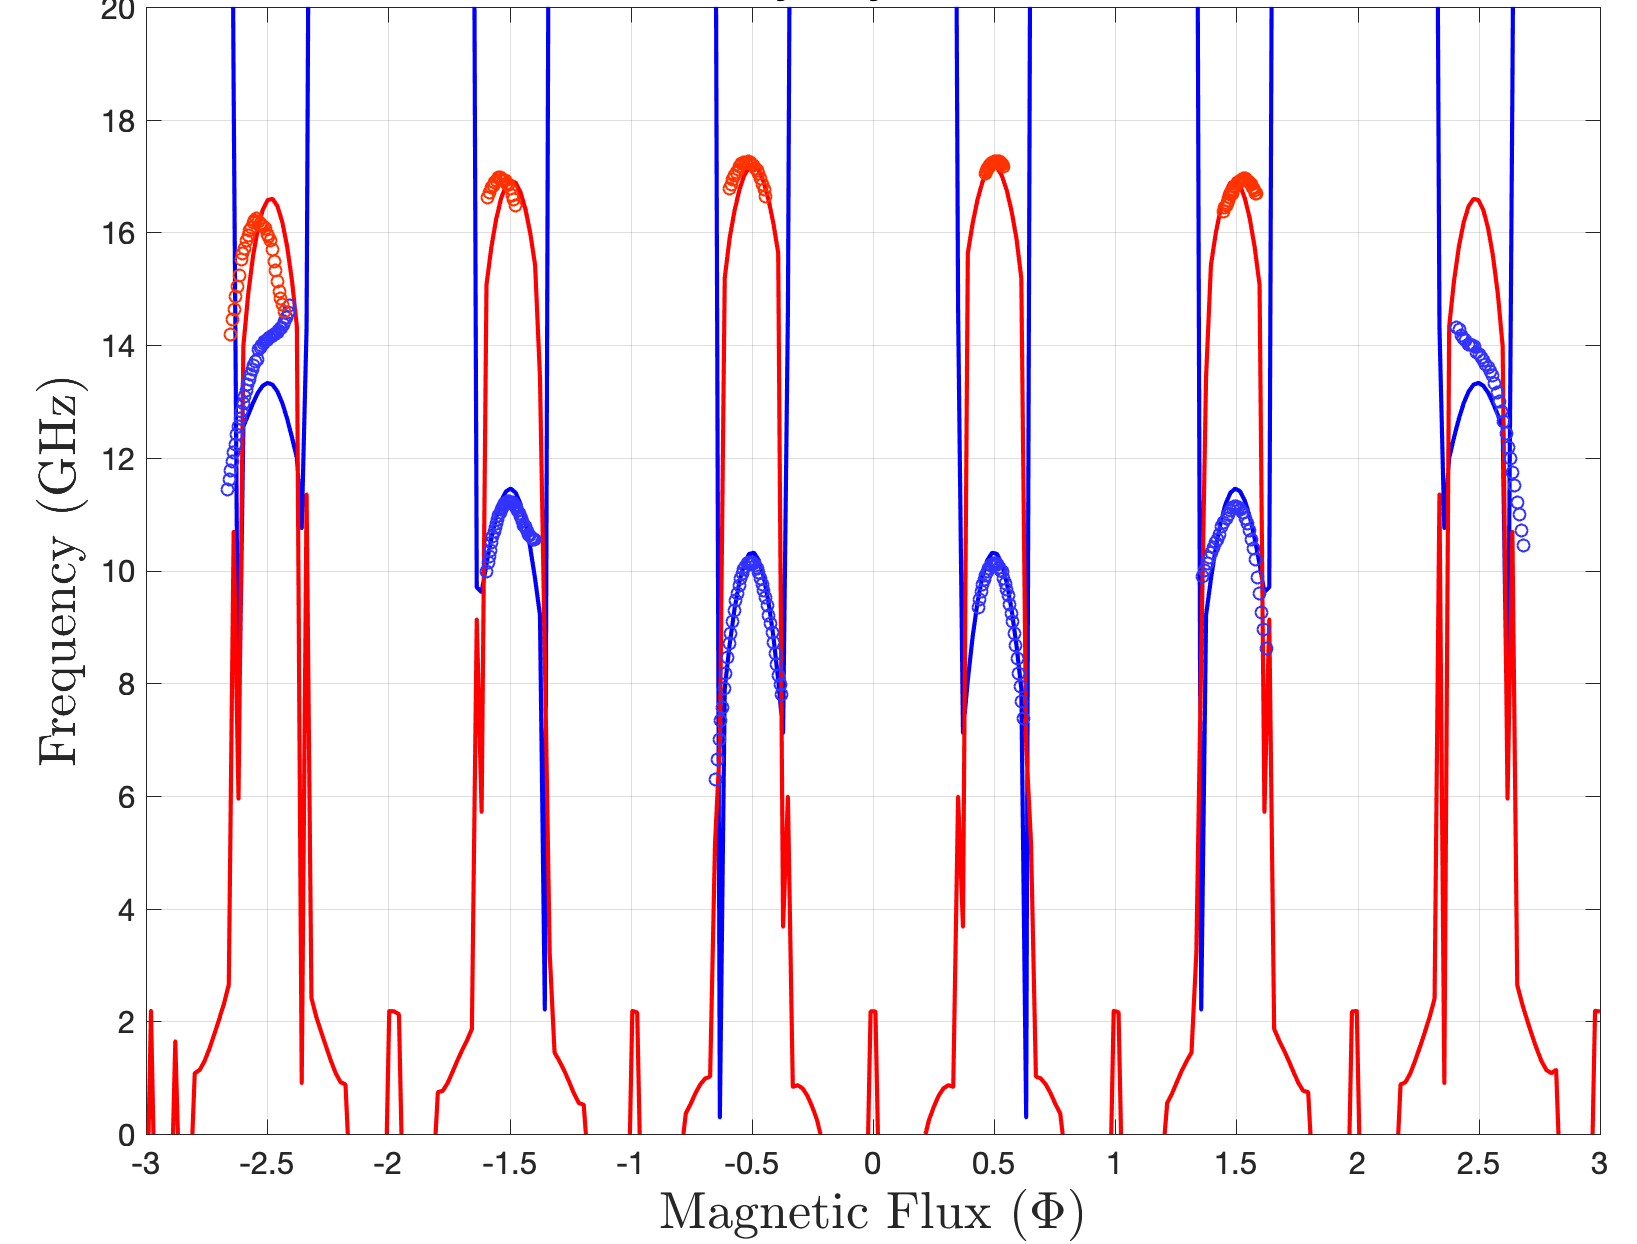
\includegraphics[height = 6cm]{figure3_qubit2}
% %            \caption{Experimental          results         were          fitted          with
% %   $  E_J =  \iunit{91}{GHz}, E_C =  \iunit{13.5}{GHz}, \alpha =  \iunit{1.023}{} $,  (compared to
% %   \iunit{E_C = 10}{GHz}, \iunit{E_J=16}{GHz},  \iunit{\alpha = 1.05}{} expected from fabrication)
% %     and   an   assymetry  between   the   areas   of   the   loops   of  $   1.011   $   was
% %   introduced. \label{fig:simulation}}
% % \end{figure}

% % We attribute this to the equilibrated bias flux that is applied to the twin loops - a change
% % in flux will \includeref{mathematical proof here}.

% % \includeref{Phase is not localised, due to infinite cosine potential.}
% % Special thank  you to  the new clean  room and  my motivation of  confronting the  dragon of
% % chaos.
